\section{Motivation}
\label{idea-sec-motivation}

IDEA's architecture is motivated by two observations about current sensor
networks. First, many sensor network applications require a large portion of
the network to meet their fidelity requirements. Because of this, a network
with 50\% of its nodes online is likely providing a much lower application
fidelity. The non-linear relationship between node availability and
application fidelity is exacerbated by the fact that frequently the most
heavily-loaded nodes are so precisely because they are being used to meet
application requirements. When they are lost, the aggregate performance of
the entire network is severely impacted.

Second, a portion of the load at each node is due to interaction with other
nodes. This load cannot be reduced unilaterally. Instead, its reduction must
be negotiated with the external nodes producing the load. A node with a
valuable sensor input may do everything possible locally to reduce its power
consumption, but unless it can move itself off of a high-traffic routing path
a large portion of its energy will be consumed by routing data.  

Existing approaches to sensor network energy management suffer from several
weaknesses. Attempts to perform local energy minimization assume that each
node lowering its own power consumption is best for the network as a whole.
However, this is not always the case. Such approaches also cannot address
the external load problem described above. Some sensor network
protocols embed forms of distributed energy management into their operation,
but by doing so they encode policies unsuitable for certain
applications. IDEA addresses these deficiencies by providing a distributed
service allowing any component controlling distributed load to perform
collaborative energy management.

\subsection{Example: Energy-Aware Routing}

\begin{figure}[t]
\label{idea-fig-motivationexample}
\begin{center}
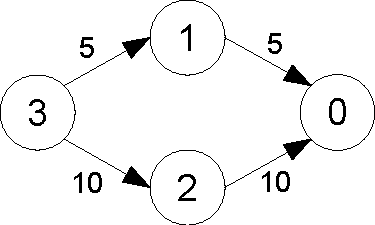
\includegraphics[width=0.6\hsize]{./7-idea/figs/MotivationExample.pdf}
\end{center}
\caption{\textbf{Example simple routing problem.}}
\end{figure}

As a simple example demonstrating the need for IDEA, consider a four-node
routing problem.  Figure~\ref{idea-fig-motivationexample} shows the network
topology, with the energy required to reliably transfer a packet over each
link shown. (To simplify the example we ignore receive costs and assume a
powered sink.) The application attempts to localize events by collecting data
from the network, and must use all four nodes, meaning that the loss of a
single node will render the network useless.

Node 3 has two routes to the sink Node 0: $3,1,0$ and $3,2,0$. If Node 3
conserves power by making a local greedy decision, it will route through Node
1, since sending a packet to Node 1 consumes $5$ units of energy as opposed
to $10$ units for sending to Node 2. Even assuming Node 3 knows the power
consumption of the links $1,0$ and $2,0$, with no other information it still
chooses the route though Node 1, which consumes less total energy per packet
than the route through Node 2, 10 units per packet versus 20 units.

The question we ask is, under what conditions will using route $3,1,0$ ---
which consumes the least energy locally and globally --- actually
\textit{harm} application performance?  We identify four situations where
using the alternative route $3,2,0$ is the correct choice, each described
below. To facilitate our discussion we define $B_n$, $C_n$ and $L_n$ as the
battery, charging rate and non-routing load at Node $n$ respectively. The
choice we are considering is between two possible load distributions, $R \in
\mathcal{R}$, where $R^{3,1,0} = [0, 10, 10, 10]$ and $R^{3,2,0} = [0, 5, 20,
10]$.  $R^{Route}_n$ represents the network-wide cost per transfer to Node
$n$ assuming Node 3 uses the route indicated.  (Nodes 1 and 2 route directly
to the sink.)

\begin{itemize}

\item \textbf{Differences in initial battery levels:}\\If the nodes are not
harvesting energy ($C_n = 0 \forall n$), no non-routing load
exist ($L_n = 0) \forall n$), and Nodes 2 and 3 have significant more energy
than Node 1, then routing through Node 2 will increase the lifetime of Node
1, which due to its low battery level defines the lifetime of the entire
network. Specifically, if $B_2 > B_1 * 2$ and $B_3 > B_1 * 2$  then using
$R^{3,2,0}$ will increase the useful lifetime of the network.

\item \textbf{Differences in non-routing load rates:}\\Assuming equal initial
energy availability and no harvesting, consideration of non-routing load
$L_n$ is similar to differences in battery sizes. Differences in non-routing
load rates between the nodes could be due to higher sampling rates or sensor
energy costs on various nodes. Assuming $B_n = \beta$ $\forall n$ and $C_n =
0$ $\forall n$, the result is similar: if $L_2 + 10 \le L_1 - 5$ and $L_3 + 5
\le L_1 - 5$ then using $R^{3,2,0}$ will increase the network's lifetime.

\item \textbf{Differences in charging rates:}\\If $C = [0, 20, 20, 20]$, then
both routes allow all nodes to continue to charge, but $R^{3,1,0}$ leads to
an aggregate charging rate of $40$ whereas $R^{3,2,0}$  produces an
aggregate charging rate of only $25$, leaving $R^{3,1,0}$ the better option.
However, if $C = [0, 5, 20, 20]$, then the application must choose between
the lower aggregate charging rate of $15$ but better survivability of
$R^{3,2,0}$ and the higher aggregate charging rate of $25$ but
unsustainability of $R^{3,1,0}$.  Since our application cannot tolerate the
loss of a single node, it chooses the lifetime of Node 1 over charging at
Nodes 2 and 3, and thus $R^{3,2,0}$.  Note that if $C = [0, 5, 10, 10]$, then
no $R \in \mathcal{R}$ leads to a non-zero charging rate and the best route
is again $R^{3,1,0}$.

\item \textbf{Overcharging:}\\Assuming that the batteries at Nodes 2 and 3
have reached capacity, but Node 1 has not, if $R^{3,2,0}_2 > C_2$ and
$R^{3,2,0}_3 > C_3$ then using $R^{3,2,0}$ will either increase the charging
rate at Node 1, if it is charging, or increase its lifetime by reducing its
load if it is not. Either outcome is beneficial to the application.

\end{itemize}

Making the correct decision at Node 3 in all four cases requires that it know
the load rates, charging rates and battery levels at Nodes 1 and 2. IDEA
addresses this problem by distributing this information. In addition, by
considering each case we can motivate some of the principles of the
distributed energy load management that IDEA enables. The network may want to
shift load \textit{towards} nodes that have a great deal of stored energy,
low load rates, high charging rates, or charging energy currently
going to waste, and \textit{away} from nodes with low batteries, low
charging rates, or that are already highly-loaded. In cases where shifting
load produces extra overall load for the network, as it does above, changes
in load distribution must be managed by the application based on
its own goals and requirements. Had our application above been able to
tolerate the loss of Node 1 it might have chosen to optimize charging at
Nodes 2 and 3 in the third example. Respecting these differences, IDEA
is built to facilitate application-level input into its decision-making
process, in order to allow solutions tailored to different fidelity
requirements.

